
% GRADING RUBRIC:
% Task definition: is the task precisely defined and does the formulation make sense?
% Approach: was a baseline, an oracle, and an advanced method described clearly, well justified, and tested?
% Data and experiments: have you explained the data clearly, performed systematic experiments, and reported concrete results?
% Analysis: did you interpret the results and try to explain why things worked (or didn't work) the way they did? Do you show concrete examples?


\documentclass[journal]{IEEEtran}
\usepackage{graphicx, amsmath, amssymb, epstopdf}
\usepackage{graphicx}
\usepackage{url}

% correct bad hyphenation here
\hyphenation{op-tical net-works semi-conduc-tor}


\begin{document}
\title{Predicting movie ratings}

\author{Carolyn~Au~\IEEEmembership{auc@stanford.edu},
        Justin~Cunningham~\IEEEmembership{jcnnghm@stanford.edu},
        and~Weixiong~Zheng~\IEEEmembership{zhengwx@stanford.edu}}

\markboth{CS 221 (Autumn 2014) Project Final Report}%
{}

\maketitle


\begin{abstract}
The project aims to explore machine learning methods to predict a movie's critical success prior
to it's release, i.e. based solely on metadata available about the movie. The code for this project
can be found at \texttt{\url{https://github.com/jcnnghm/cs221-project}}
\end{abstract}


\section{Overview}
The movie industry generates multi-billion dollars in revenue and most movies
cost millions of dollars to create.  However, not all movies are successes.
With such high risk and large amounts of money involved, it would be useful to
be able to predict the success of a movie before it is released. In this
project, we try to predict the critical success of a movie, as shown by user
ratings on IMDb \cite{imdb}, based solely on metadata about a movie available prior to it's
release.

\begin{itemize}
    \item Input: IMDb metadata for a movie related to it's creation and release
    \item Output: Predicted user rating of a movie, on a scale of 0-10
\end{itemize}


\section{Related Work}
Henning-Thurau, Houston and Walsh \cite{marketing} performed an empirical study
to distinguish direct and indirect relationships among different determinants
of movie success and found that star and director power does not guarantee
success. However, cultural familiarity (e.g. sequels to a successful movie),
release dates (e.g. during the summer), budget and awards were a huge predictor
of success. Relatedly, Deniz and Hasbrouck \cite{greenlight} performed
statistical analysis on the top 150 grossing movies of 2010 and found that
genre, MPAA rating, budget, star power, adaptation from another medium, sequels
and remakes are significant predictors
of box office revenue. 
\\
\par There are also other student projects that attempted to predict user
ratings. One was done for the Machine Learning class (CS229) \cite{hitorflop},
where they used Naive Bayes and Support Vector Machines to predict IMDb user
ratings and profitability. Their system performed moderately well on their test
data. Another similar project \cite{cooper} used regression (Support Vector
Regression, Boosted Decision Trees, Gradient Boosting Regression and Random
Forest Regression) over a different dataset (The Sagel Index of the top and
worst 1000 films), predicting audience ratings on Rotten Tomatoes. Their system
resulted in error rates of roughly 10\%.

\section{Dataset}
Our dataset is the list of all movies from IMDb that fulfill the following properties
\begin{itemize}
	\item Released in the US
	\item Generated gross earnings in the US
	\item Has at least 1,000 user votes to rate the movie
\end{itemize}

\par After pruning the database of 3 million entries, we are left with 9,888
movies which is a reasonable number for our algorithms to run on. Limiting the
data to movies with a reasonable number of user votes also ensures that the
rating data is not too noisy. We save 20\% of the data for testing, and use the
rest for development.

\scalebox{0.55}{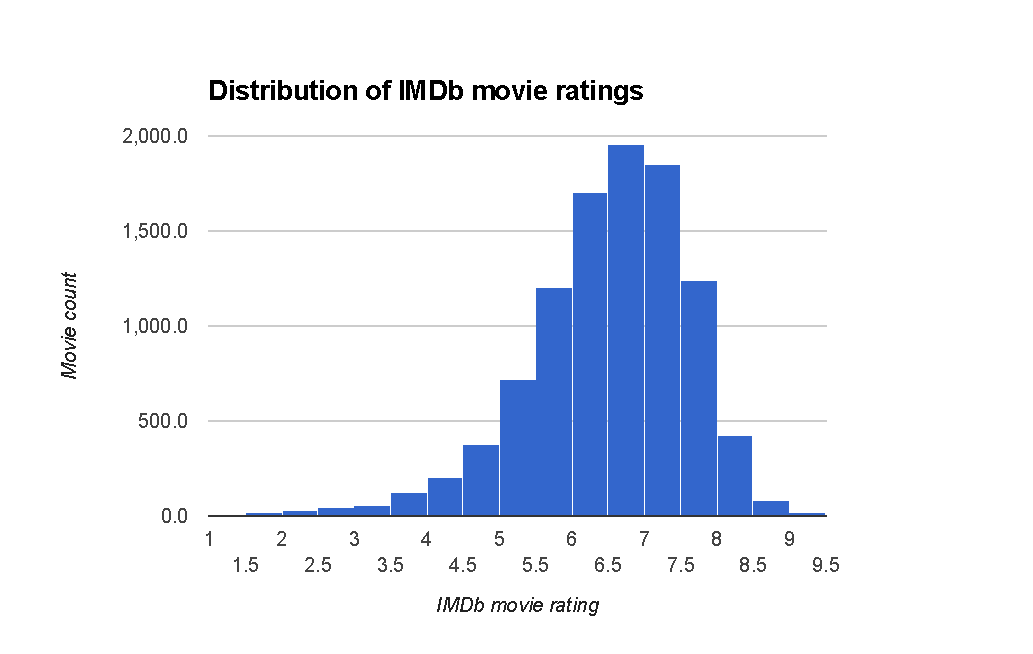
\includegraphics{ratings.eps}}

The user ratings in our dataset have a mean of 6.5 and a median of 6.6 with a standard deviation of 1.05.

\section{Evaluation Metric}
We used the standard deviation of the predicted user rating from the actual values on IMDb, calculated as

$$ \sqrt{\frac{\sum_{i=1}^n(\text{Predicted}_i-\text{Actual}_i)^2}{n}} $$

\subsection{Baseline}
For our baseline, we included the following features:
\begin{itemize}
	\item Complete cast members, which includes actors, directors, producers, etc.
	\item Movie genre
	\item Keywords describing the movie
\end{itemize}

This results in a sample standard deviation of 0.06 on the training data, and
1.78 on the test data.

\subsection{Oracle}
For our oracle, we added additional features which are movie data available
\emph{after} a movie is released. These are:
\begin{itemize}
	\item Gross earnings
	\item IMDb user ratings
	\item Number of votes for the ratings
\end{itemize}

This results in a sample standard deviation of of 0.03 on the training data, and 0.34 on the test data.
\\
\par We had initially added critic and audience ratings from Rotten Tomatoes, but it produced unexpected results, namely critic scores were negative weights and negative audience ratings had the opposite effect (movies rated \emph{Spilled} had larger weights than \emph{Upright})

\section{System design}
Our system is composed of a feature creator system, a snapshot of the IMDb dataset,
and a variety of learning algorithms that operate on the information exported by
the feature creator.
\par The feature creator provides a framework that allows sub-component
feature extractors to interact with the IMDb dataset, stored in MySQL.  The feature
creator calls each extractor ($E_i$ in the diagram below) in turn for each of the movies we've selected for our
dev and test sets, and merges their output features into a sparse feature vector for
each movie.  An additional combinator step ($C_i$ in the diagram) is applied to generate feature
combinations, e.g. \{movie director $\times$ movie actors\}.
\par The creator is highly configurable so that extractors and combinators can easily be selectively enabled or disabled,
and includes a caching layer to reduce the load on MySQL and speed up processing.
The feature vectors are stored in JSON so that they can be easily
post-processed for use with different algorithms. \\

\begin{center}
    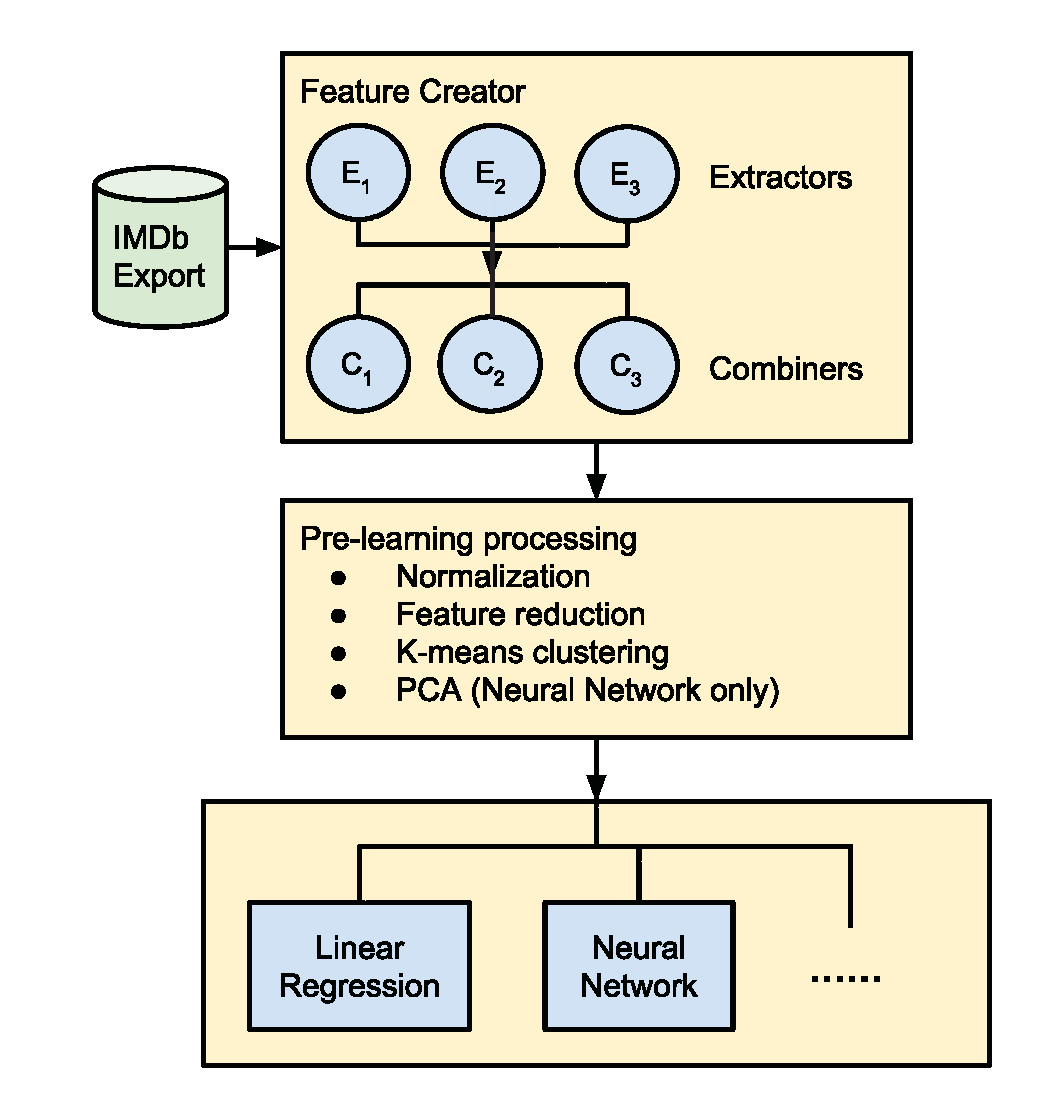
\includegraphics[width=8cm]{charts/system.eps}
\end{center}

Each algorithm is responsible for transforming the data to the format that it requires.
The neural network, for example, converts the sparse vectors from the feature creator
into a dense representation that can be consumed by FANN \cite{fann}, a neural network library.  Each
component is modular, so that it is easy to tune individual algorithms.


\section{Features}
The feature creator system extracts raw features, and then combines some
features with others, like actors with directors, to form compound
"combination" features, e.g. \{movie director $\times$ movie actors\}.
Below is a detailed description of each class of features we include along with
an example of the features we generate.

\subsection{Individual features}
\subsubsection{Budget}
The Budget feature extractor extracts a weighted feature, within the domain of
\$1 to \$300M.  Since the data is crowdsourced, there are multiple specified
budgets for the movie.  We only consider movies with budgets in US dollars, and
we take the largest proposed budget.  We also consider using budgets in two
ways -- using raw dollar values or bucketing the value into \$5M chunks (as
indicator variables).

\begin{align*}
        \{ \ \ & \\
        &``budget": 10000000,\\
        &``budget\_bucket\_2: 1\\
        \} \ \ &
\end{align*}

\subsubsection{Cast}
The cast feature extractor generates indicator features for each
cast and crew member associated with a film, for each job they 
performed.  An individual could potentially appear more than once,
if they performed different jobs, for example, if they were both
an actor and director.  The cast roles which we include are:
\begin{itemize}
	\item Actor
	\item Actress
	\item Producer
	\item Writer
	\item Cinematographer
	\item Composer
	\item Costume designer
	\item Director
	\item Editor
	\item Production designer
	\item Miscellaneous crew
\end{itemize}

\begin{align*}
        \{ \ \ & \\
        &``Lasseter,John\_producer": 1,\\
        &``Cummings,Jim\_actor": 1,\\
        &``Mitchell,Nicole\_writer": 1,\\
        \} \ \ &
\end{align*}

\subsubsection{Genre}
Genre features are indicator features that are activated for each
genre associated with a movie in the IMDb dataset.

\begin{align*}
        \{\ \ &\\
        &``genre\_Family": 1,\\
        &``genre\_Comedy": 1,\\
        \}\ \ &
\end{align*}

\subsubsection{Keywords}
Keyword features are indicator features that are activated for
each searchable tag that is associated with a movie in the
IMDb dataset.

\begin{align*}
        \{\ \ &\\
        &``character-name-in-title": 1,\\
        &``sequel": 1,\\
        &``friendship": 1,\\
        \}\ \ &
\end{align*}

\subsubsection{Release Date}
Release dates are also indicator features that are activated for each release
in the US across festivals and premieres. For each release, we generate 3
features, one for the month, year, and both month and year.

\begin{align*}
        \{\ \ &\\
        &``release\ (traverse\ film\ festival)\ (August)": 1, \\
        &``release\ (traverse\ film\ festival)\ (2014)": 1, \\
        &``release\ (traverse\ film\ festival)\ (August\ 2014)": 1, \\
        &``release\ (premiere)\ (February)": 1, \\
        &``release\ (premiere)\ (2014)": 1, \\
        &``release\ (premiere)\ (February\ 2014)": 1, \\
        \}\ \ &
\end{align*}

\subsubsection{Budget $\times$ Cast}
We use the bucketized budget data and join that with the extracted cast
features. The idea is that an actor's star power will be amplified by a big
budget production, or reduced in an indie movie.

\begin{align*}
        \{\ \ &\\
        &``budget\_bucket\_2\_Cummings,Jim\_actor": 1,\\
        &``budget\_bucket\_2\_Klein,Sebastian\_actor": 1\\
        \}\ \ &
\end{align*}

\subsubsection{Actor $\times$ Director}
We create new features for each combination of actor and director in each cast
list (where actor includes both actors and actresses, treated distinctly in our
dataset). The intuition is that some pairs of actors and directors work well
together and create better movies together.

\begin{align*}
        \{\ \ &\\
        &``Nolan,Christopher\_Cummings,Jim\_actor": 1,\\
        &``Nolan,Christopher\_Klein,Sebastian\_actor": 1\\
        \}\ \ &
\end{align*}

\subsubsection{Standardized budget}
In order to account for inflation, we added a feature which calculates the
standard score of the movie budget based on other movies released that same
year.  The standard score of the movie budget for a movie $M$ released in year
$Y$ is given by

\begin{eqnarray*}
    z = \frac{x - \mu}{\sigma}
\end{eqnarray*}
where
\begin{itemize}
    \item $z$ is the standard score of the budget for movie $M$
    \item $\mu$ is the mean of movie budgets released in year $Y$
    \item $\sigma$ is the standard deviation of movie budgets released in year $Y$
\end{itemize}
\begin{align*}
        \{\ \ &\\
        &``standardized_budget": 0.57408881370714016,\\
        \}\ \ &
\end{align*}

\subsubsection{Actor experience}

\subsection{Analysis of feature sets}
In total, there are about 192,000 unique features without combined features for
our data set.  With combined features, this number balloons to over 800,000.

\scalebox{0.55}{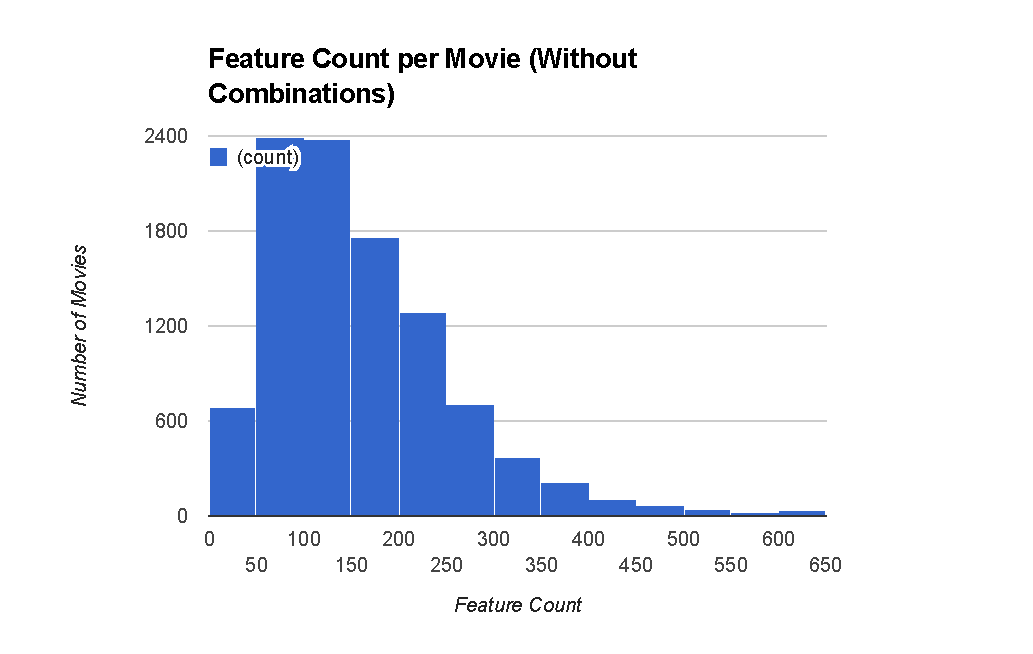
\includegraphics{charts/features_without_cross_chart.eps}}

\scalebox{0.55}{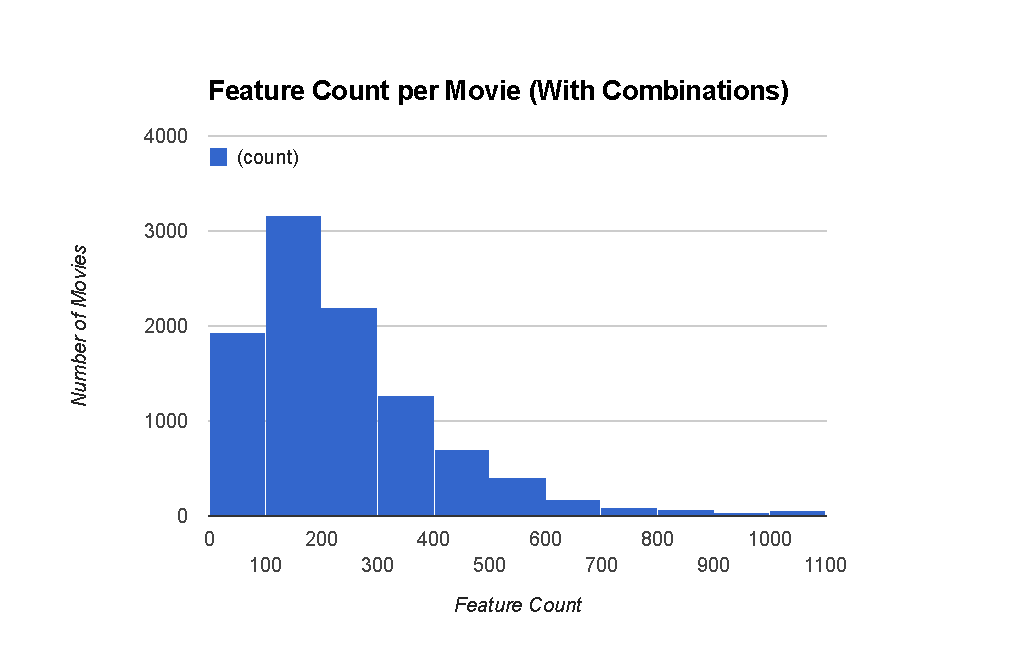
\includegraphics{charts/features_with_cross_chart.eps}}

When represented sparsely, the feature size without combinations is about 53MB, and 82MB with combinations.  The same data represented
densely consumes approximately 3.5GB and 14GB respectively, indicating that many of the features are not associated with many movies.  Features are associated with an average of 8 movies, skewed heavily to the left. \\
\\
\scalebox{0.50}{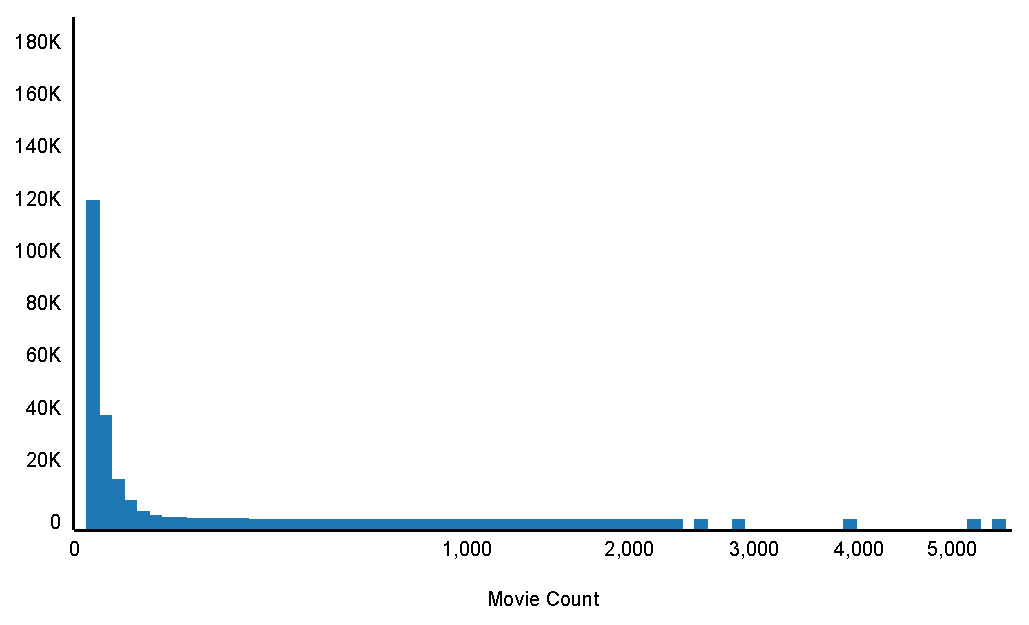
\includegraphics{charts/movies_per_feature.eps}}
\\
\par An initial investigation into the importance of each feature was performed by
running our baseline algorithm with each feature set individually.\\
\\
\begin{tabular}{|l|r r|} % columns
\hline
Feature & Dev error & Test error \\ [0.5ex] % inserts table 
\hline % inserts single horizontal line
Budget (raw) & 5.89 & 5.87 \\ % inserting body of the table
Budget (bucketized) & 4.62 & 4.68 \\
Cast & 0.65 & 2.56 \\
Genre & 2.26 & 2.29 \\
Keywords & 1.65 & 3.35 \\
Release date & 1.69 & 2.26 \\
\hline
Budget $\times$ Cast & 4.54 & 5.65 \\
Actor $\times$ Director & 2.67 & 5.96 \\
\hline
Standardized budget & 5.02 & 5.03 \\
Cast experience & $\infty$ & $\infty$ \\
\hline
\end{tabular}
\smallskip
\par Here we note that some feature sets are overfitted to our dev dataset such as
cast, keywords, release date, budget $\times$ cast and actor $\times$ director.
These are also our largest feature sets.\\
\\
\begin{tabular}{|l| r r r|} % columns
\hline
Feature             & \shortstack[c]{Num.\\vars} & \shortstack[c]{Num.\\movies} & \shortstack[c]{Feature / \\ movie}  \\ [0.5ex] % inserts table 
\hline
Budget (raw)        & 1 & 5,278 (53\%) & 1 \\ % inserting body of the table
Budget (bucketized) & 52 & 5,278 (53\%) & 1 \\
Cast                & 169,973 & 9,883 (99\%) & 72 \\
Genre               & 25 & 9,885 (99\%) & 2 \\
Keywords            & 11,701 & 9,774 (98\%) & 75 \\
Release date        & 10,500 & 9,884 (99\%) & 7 \\
\hline
Budget $\times$ Cast & 394,661 & 5,278 (53\%) & 92 \\
Actor $\times$ Director & 282,672 & 8,630 (87\%) & 35 \\
\hline
Standardized budget & 1 & 5,278 (53\%) & 1 \\
Cast experience & $\infty$ & $\infty$ & $\infty$ \\
\hline %inserts single line
\end{tabular}

\subsection{Feature pruning}
With combined features, our feature space size is around 800,000. It takes hours to train a Linear Regression Model using scikit-learn \cite{scikit} on such a large sample space. We did some experiments on feature removal to improve algorithm performance.
\par In our experiments, we removed all the features that appear less or equal to $n$ times in the training data before training a model. We measured the number of features left after removal and the standard error on test set.\\
\\
\begin{tabular}{|l| r r|} % columns
\hline
$n$ & Num. features left & Standard Error  \\ [0.5ex] % inserts table 
\hline
0 & 723,000 & N/A \\
1 & 188,000 & 0.79 \\
2 & 93,000  & 0.83 \\
9 & 28,000  & 1.12 \\ [1ex]
\hline %inserts single line
\end{tabular}
\smallskip
\\
\textit{delete or update this paragraph?}
\par Removing the features that
appear only once in the training set gives huge improvements on performance
while maintaining low standard errors on fitting the test set. This makes sense
because if a
feature appears only once in the training set, it's highly likely that the
feature won't appear in the test set, which means that the weight for this feature
won't affect the result of fitting the test set. Also, according to the experiment,
increasing the threshold $n$ doesn't give too much performance gain but worsens
the test error.

\subsection{Principal Component Analysis}
We ran Principal Component Analysis, PCA, on our features to further analyze
the data, and to reduce our feature size for the neural network. With PCA, we
are able to reduce our feature set to 5,000.  It shows that the first feature
represents about 1.5\% of the variance.  Further, the first 5,000 features
capture 91\% of the variance from the data.
\\
\scalebox{0.575}{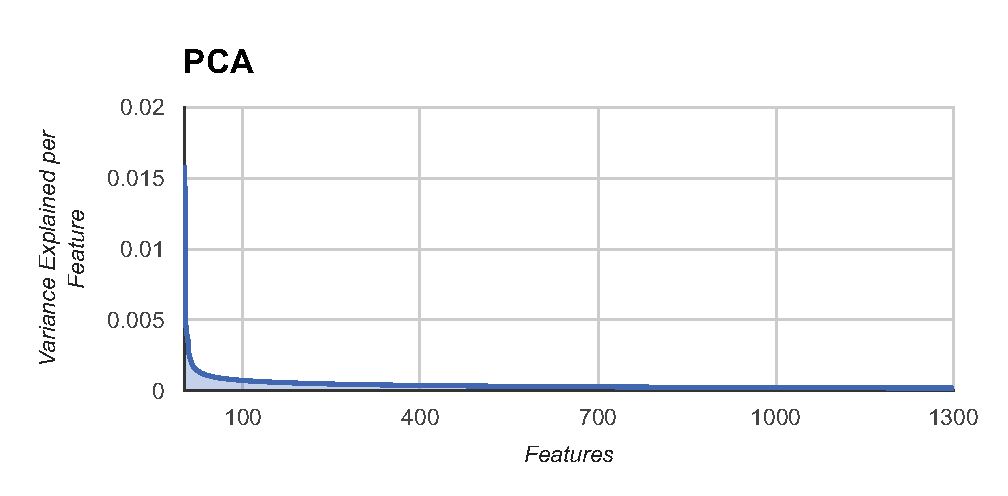
\includegraphics{charts/pca.eps}}
\\
\scalebox{0.55}{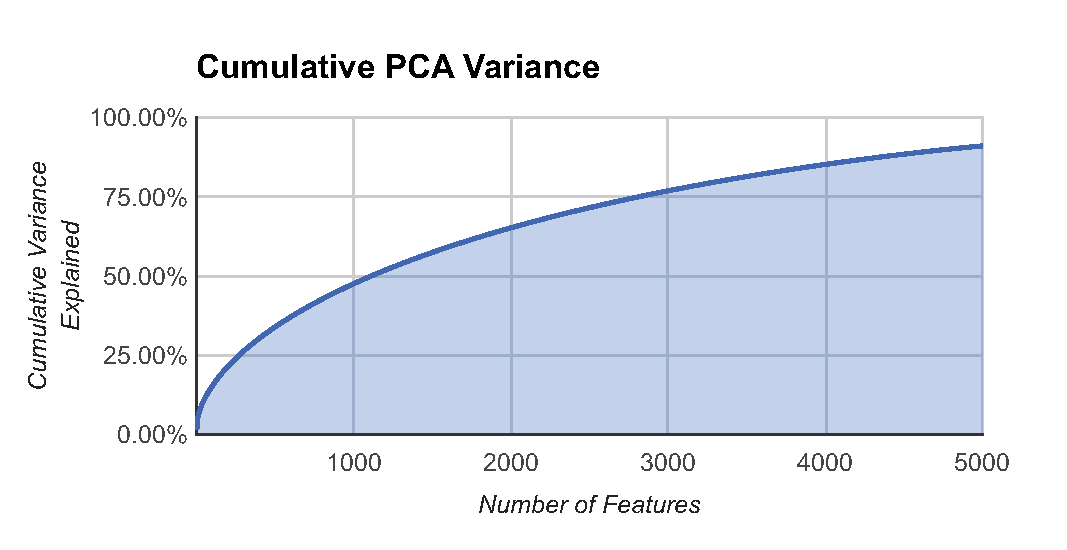
\includegraphics{charts/pca_variance.eps}}

\subsection{K-means}

\section{Algorithms}

\subsection{Linear Regression}
We used the implementation of Linear Regression in scikit-learn with default
parameters. We used feature removal threshold 1. The algorithm took 2.4 hours
to run and gave standard error 0.79.

\subsubsection{Regularization}

\subsection{Logistic Regression}

\textit{Maybe we should just skip this, we didn't cover it in class and it didn't perform better than anything else.}

\subsection{SVM}
We used the implementation of SVM in scikit-learn with radial basis function (rbf) kernel and linear kernel. We used the feature removal threshold of 1. SVM with rbf kernel took 3.3 hours to run and gave standard error of 1.09. SVM with linear kernel took 3 minutes to run and gave standard error of 1.02.

\subsection{Neural Network}
The neural network is implemented using the Fast Artificial Neural Network (FANN)
API.  With two hidden layers, with 20 neurons in the first and 10 in the second, 
we have achieved a test error rate of 0.012, when the rating is represented as a
number between 0 and 1.0, corresponding to an average error of approximately 1.1 out of 10.  

The neural network is slow to learn, so we plan to reduce the number of features so we can
iterate more quickly.  In addition, we plan to tune the network topology once we're able
to achieve acceptable iteration speeds.

\section{Results}
\smallskip
\begin{tabular}{|l |l l|} % columns
\hline
Model               & Time to fit & Standard Error  \\ [0.5ex] % inserts table 
\hline
Neural network      & $>$ 10 hours  & 1.1 \\
Linear regression   & 2.4 hours   & 0.79 \\
SVM (rbf kernel)    & 3.3 hours   & 1.09 \\
SVM (linear kernel) & 3 minutes   & 1.02 \\ [1ex]
\hline %inserts single line
\end{tabular}
\smallskip
\\
\par The best model we have so far is Linear Regression which gives 0.79 test error.
Compare this to our baseline test error of 1.78 and oracle test error of 0.34.
We believe the improvement is mostly from feature tuning.

\section{Analysis}

\section{Acknowledgements}

% references section

% can use a bibliography generated by BibTeX as a .bbl file
% BibTeX documentation can be easily obtained at:
% http://www.ctan.org/tex-archive/biblio/bibtex/contrib/doc/
% The IEEEtran BibTeX style support page is at:
% http://www.michaelshell.org/tex/ieeetran/bibtex/
%\bibliographystyle{IEEEtran}
% argument is your BibTeX string definitions and bibliography database(s)
%\bibliography{IEEEabrv,../bib/paper}
%
% <OR> manually copy in the resultant .bbl file
% set second argument of \begin to the number of references
% (used to reserve space for the reference number labels box)
\begin{thebibliography}{1}
\bibitem{imdb}
Internet Movie Database: \texttt{\url{http://imdb.com}}

\bibitem{fann}
Fast Artificial Neural Network Library: \texttt{\url{http://leenissen.dk/fann/wp/}}

\bibitem{scikit}
Scikit-learn: \texttt{\url{http://scikit-learn.org/stable/}}

\bibitem{marketing}
H-T Thorsten, H. Mark, W. Gianfranco, \emph{Determinants of Motion Picture Box
Office and Profitability: An Interrelationship Approach} \hskip 1em plus 0.5em
minus 0.4em\relax Review of Managerial Science, 2006.

\bibitem{greenlight}
B.~Deniz and R.~B.~Hasbrouck, \emph{WHEN TO GREENLIGHT:
Examining the Pre-release Factors that Determine Future Box Office Success of a Movie in the United States}
\hskip 1em plus 0.5em minus 0.4em\relax International Journal of Economics and Management Sciences, 2012.

\bibitem{hitorflop}
D.~Cocuzzo and S.~Wu, \emph{Hit or Flop: Box Office Prediction for Feature
Films}\hskip 1em plus
  0.5em minus 0.4em\relax Stanford CS 229 project, Dec 2013.

\bibitem{cooper}
S.~Mevawala and S.~Phadke, \emph{BoxOffice: Machine Learning Methods for Predicting Audience Film Ratings}\hskip 1em plus
  0.5em minus 0.4em\relax The Cooper Union for the Advancement of Science and Art.
  
\bibitem{imdb_api}
\texttt{\url{http://www.imdb.com/interfaces}}

\bibitem{rt_api}
\texttt{\url{http://developer.rottentomatoes.com}}
\end{thebibliography}

% that's all folks
\end{document}


